\section{User Interface Controls}

In this section we are going to add some supplementary controls to make the process of simulation more convenient. AnyLogic allows users to create sliders for changing the values of any parameters.

We have selected a list of parameters that are considered to be particularly important and whose values should be able to be changed during the simulation. These parameters can be seen in the following figure.

\begin{figure}[H]
  \centering
  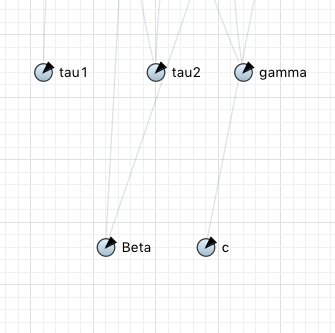
\includegraphics[height=0.4\textwidth]{img/screens/sliders/sliders1}
  \caption{Sensitive parameters of the model}
\end{figure}

A slider element can be created by using the user interface of the AnyLogic application. We create a slider for $\tau_1$ parameter and put it near the parameter element. The slider is connected with the variable.

\begin{figure}[H]
  \centering
  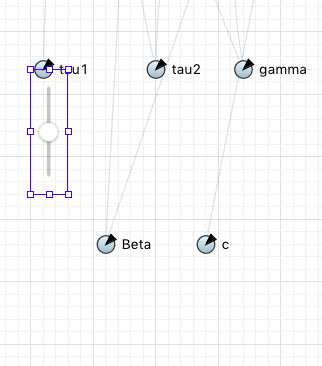
\includegraphics[height=0.4\textwidth]{img/screens/sliders/sliders2}
  \caption{Creating a slider for $\tau_1$}
\end{figure}

If we look in the properties window, we will find out that sliders have their own custom properties. There is the name of the parameter that the slider is linked to, the minimum and maximum possible values.

\begin{figure}[H]
  \centering
  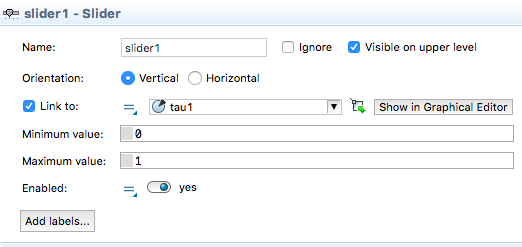
\includegraphics[height=0.3\textwidth]{img/screens/sliders/sliders7}
  \caption{Properties of $\tau_1$ slider}
\end{figure}

For all parameters selected by us as being particularly important, we create the sliders exactly the same way that we did with the first one. Here, each parameter will have the corresponding slider near the located variable.

\begin{figure}[H]
  \centering
  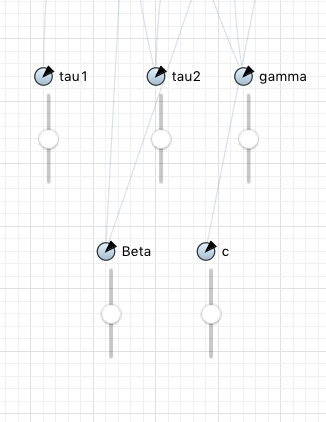
\includegraphics[height=0.5\textwidth]{img/screens/sliders/sliders3}
  \caption{Created sliders for all sensitive parameters}
\end{figure}

The value of $\beta$ can change depending on the society being observed. The spatial characteristic of the hospital's building is also important, as it may affect the rate of contacts between different patients and medical workers. The value of our contact rate will vary from 0 to 4.

\begin{figure}[H]
  \centering
  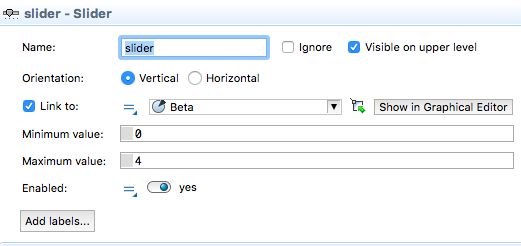
\includegraphics[height=0.3\textwidth]{img/screens/sliders/sliders6}
  \caption{Properties of $\beta$ slider}
\end{figure}

The parameter $c$ is one of the key parameters that has much influence on the population infected by resistant bacteria. Since it represents a portion of a flow, it will vary between 0 and 1. When $c$ is zero, the InfectionR flow will not differ from the infectionS flow, and approaches zero as $c$ approaches to 1.

\begin{figure}[H]
  \centering
  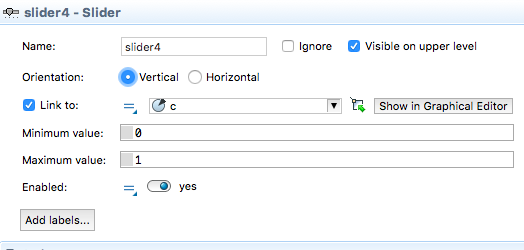
\includegraphics[height=0.3\textwidth]{img/screens/sliders/sliders8}
  \caption{Properties of $c$ slider}
\end{figure}

Occasional recovery from both bacteria strains occur with rate $\gamma$ in our system. Since it represents a probability, the value always lies between 0 and 1. However to make the slider less sensitive for changes, we set its minimum and maximum values to be 0.01 and 0.10 respectively.

\begin{figure}[H]
  \centering
  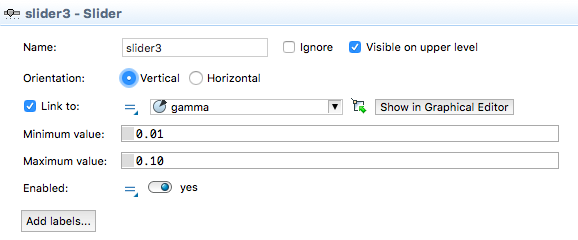
\includegraphics[height=0.3\textwidth]{img/screens/sliders/sliders9}
  \caption{Properties of $\gamma$ slider}
\end{figure}

The slider that have been created allow the user to change the value of a particular parameter during the simulation process and see how it affects the flow in the system. The model execution in AnyLogic displays the actual value of a parameter near its name.

\begin{figure}[H]
  \centering
  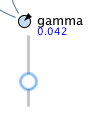
\includegraphics[height=0.2\textwidth]{img/screens/sliders/sliders5}
  \caption{Updating the slider value during the model execution}
\end{figure}

By dragging the slider, the user can change the value of each parameter between its predefined minimum and maximum values.
